% Created by tikzDevice version 0.12.6 on 2026-08-08 02:45:01
% !TEX encoding = UTF-8 Unicode
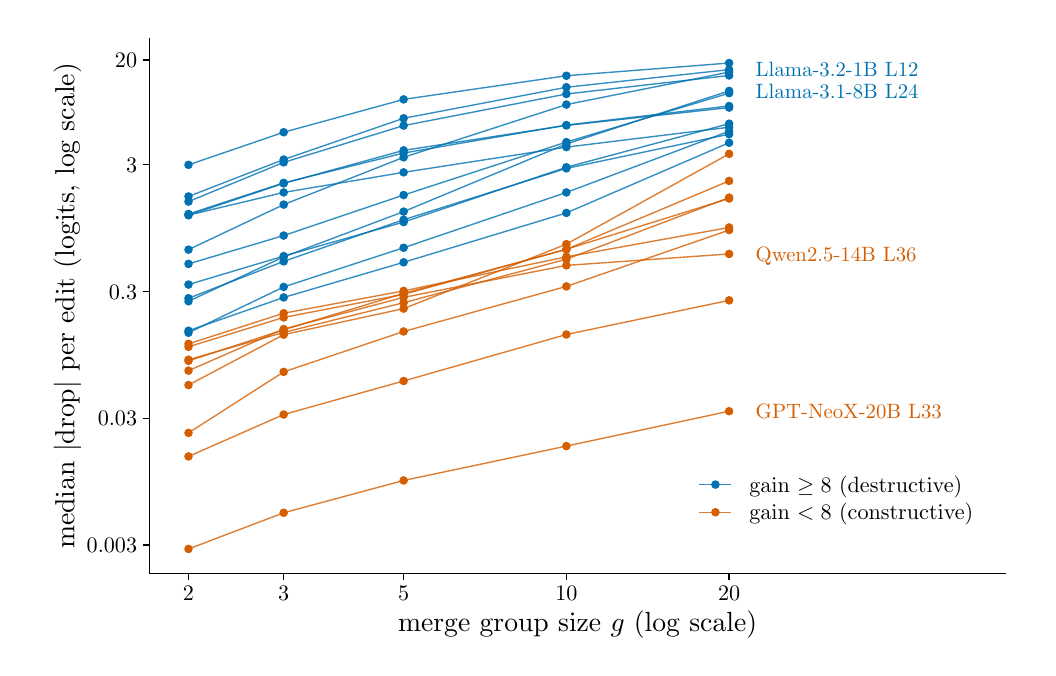
\begin{tikzpicture}[x=1pt,y=1pt]
\definecolor{fillColor}{RGB}{255,255,255}
\path[use as bounding box,fill=fillColor,fill opacity=0.00] (0,0) rectangle (361.35,224.04);
\begin{scope}
\path[clip] (  0.00,  0.00) rectangle (361.35,224.04);
\definecolor{drawColor}{RGB}{255,255,255}
\definecolor{fillColor}{RGB}{255,255,255}

\path[draw=drawColor,line width= 0.5pt,line join=round,line cap=round,fill=fillColor] (  0.00,  0.00) rectangle (361.35,224.04);
\end{scope}
\begin{scope}
\path[clip] ( 44.05, 26.90) rectangle (353.35,220.04);
\definecolor{fillColor}{RGB}{255,255,255}

\path[fill=fillColor] ( 44.05, 26.90) rectangle (353.35,220.04);
\definecolor{drawColor}{RGB}{0,114,178}

\path[draw=drawColor,draw opacity=0.80,line width= 0.5pt,line join=round] ( 58.11,156.30) --
	( 92.51,164.50) --
	(135.85,171.76) --
	(194.66,180.87) --
	(253.46,188.06);

\path[draw=drawColor,draw opacity=0.80,line width= 0.5pt,line join=round] ( 58.11,156.71) --
	( 92.51,167.94) --
	(135.85,178.74) --
	(194.66,188.84) --
	(253.46,195.74);

\path[draw=drawColor,draw opacity=0.80,line width= 0.5pt,line join=round] ( 58.11,156.29) --
	( 92.51,167.78) --
	(135.85,179.70) --
	(194.66,188.72) --
	(253.46,195.16);
\definecolor{drawColor}{RGB}{213,94,0}

\path[draw=drawColor,draw opacity=0.80,line width= 0.5pt,line join=round] ( 58.11, 35.68) --
	( 92.51, 48.75) --
	(135.85, 60.42) --
	(194.66, 72.84) --
	(253.46, 85.45);

\path[draw=drawColor,draw opacity=0.80,line width= 0.5pt,line join=round] ( 58.11,109.79) --
	( 92.51,120.85) --
	(135.85,128.93) --
	(194.66,141.23) --
	(253.46,151.84);

\path[draw=drawColor,draw opacity=0.80,line width= 0.5pt,line join=round] ( 58.11, 69.10) --
	( 92.51, 84.25) --
	(135.85, 96.37) --
	(194.66,113.16) --
	(253.46,125.50);
\definecolor{drawColor}{RGB}{0,114,178}

\path[draw=drawColor,draw opacity=0.80,line width= 0.5pt,line join=round] ( 58.11,125.17) --
	( 92.51,141.22) --
	(135.85,157.57) --
	(194.66,182.01) --
	(253.46,201.19);

\path[draw=drawColor,draw opacity=0.80,line width= 0.5pt,line join=round] ( 58.11,163.05) --
	( 92.51,176.39) --
	(135.85,191.29) --
	(194.66,202.50) --
	(253.46,208.87);

\path[draw=drawColor,draw opacity=0.80,line width= 0.5pt,line join=round] ( 58.11,174.47) --
	( 92.51,186.25) --
	(135.85,198.12) --
	(194.66,206.67) --
	(253.46,211.26);

\path[draw=drawColor,draw opacity=0.80,line width= 0.5pt,line join=round] ( 58.11,161.20) --
	( 92.51,175.36) --
	(135.85,188.65) --
	(194.66,200.08) --
	(253.46,206.76);

\path[draw=drawColor,draw opacity=0.80,line width= 0.5pt,line join=round] ( 58.11,143.83) --
	( 92.51,160.11) --
	(135.85,177.19) --
	(194.66,196.25) --
	(253.46,207.98);

\path[draw=drawColor,draw opacity=0.80,line width= 0.5pt,line join=round] ( 58.11,113.81) --
	( 92.51,130.35) --
	(135.85,144.52) --
	(194.66,164.50) --
	(253.46,186.61);

\path[draw=drawColor,draw opacity=0.80,line width= 0.5pt,line join=round] ( 58.11,114.53) --
	( 92.51,126.56) --
	(135.85,139.25) --
	(194.66,157.10) --
	(253.46,182.46);

\path[draw=drawColor,draw opacity=0.80,line width= 0.5pt,line join=round] ( 58.11,126.27) --
	( 92.51,139.59) --
	(135.85,154.64) --
	(194.66,173.19) --
	(253.46,185.55);
\definecolor{drawColor}{RGB}{213,94,0}

\path[draw=drawColor,draw opacity=0.80,line width= 0.5pt,line join=round] ( 58.11, 94.90) --
	( 92.51,113.11) --
	(135.85,122.52) --
	(194.66,145.81) --
	(253.46,178.44);
\definecolor{drawColor}{RGB}{0,114,178}

\path[draw=drawColor,draw opacity=0.80,line width= 0.5pt,line join=round] ( 58.11,138.68) --
	( 92.51,148.92) --
	(135.85,163.56) --
	(194.66,182.70) --
	(253.46,200.37);
\definecolor{drawColor}{RGB}{213,94,0}

\path[draw=drawColor,draw opacity=0.80,line width= 0.5pt,line join=round] ( 58.11,104.05) --
	( 92.51,113.92) --
	(135.85,124.65) --
	(194.66,140.39) --
	(253.46,162.63);

\path[draw=drawColor,draw opacity=0.80,line width= 0.5pt,line join=round] ( 58.11, 77.61) --
	( 92.51, 99.66) --
	(135.85,114.26) --
	(194.66,130.54) --
	(253.46,150.90);

\path[draw=drawColor,draw opacity=0.80,line width= 0.5pt,line join=round] ( 58.11,100.11) --
	( 92.51,115.13) --
	(135.85,126.59) --
	(194.66,138.14) --
	(253.46,142.27);
\definecolor{drawColor}{RGB}{0,114,178}

\path[draw=drawColor,draw opacity=0.80,line width= 0.5pt,line join=round] ( 58.11,131.22) --
	( 92.51,141.50) --
	(135.85,153.79) --
	(194.66,173.60) --
	(253.46,189.34);
\definecolor{drawColor}{RGB}{213,94,0}

\path[draw=drawColor,draw opacity=0.80,line width= 0.5pt,line join=round] ( 58.11,103.64) --
	( 92.51,114.87) --
	(135.85,128.02) --
	(194.66,143.93) --
	(253.46,168.66);

\path[draw=drawColor,draw opacity=0.80,line width= 0.5pt,line join=round] ( 58.11,108.73) --
	( 92.51,119.34) --
	(135.85,127.67) --
	(194.66,143.97) --
	(253.46,162.31);
\definecolor{drawColor}{RGB}{0,114,178}
\definecolor{fillColor}{RGB}{0,114,178}

\path[draw=drawColor,line width= 0.3pt,line join=round,line cap=round,fill=fillColor] ( 58.11,125.17) circle (  1.39);

\path[draw=drawColor,line width= 0.3pt,line join=round,line cap=round,fill=fillColor] ( 92.51,141.22) circle (  1.39);

\path[draw=drawColor,line width= 0.3pt,line join=round,line cap=round,fill=fillColor] (135.85,157.57) circle (  1.39);

\path[draw=drawColor,line width= 0.3pt,line join=round,line cap=round,fill=fillColor] (194.66,182.01) circle (  1.39);

\path[draw=drawColor,line width= 0.3pt,line join=round,line cap=round,fill=fillColor] (253.46,201.19) circle (  1.39);

\path[draw=drawColor,line width= 0.3pt,line join=round,line cap=round,fill=fillColor] ( 58.11,163.05) circle (  1.39);

\path[draw=drawColor,line width= 0.3pt,line join=round,line cap=round,fill=fillColor] ( 92.51,176.39) circle (  1.39);

\path[draw=drawColor,line width= 0.3pt,line join=round,line cap=round,fill=fillColor] (135.85,191.29) circle (  1.39);

\path[draw=drawColor,line width= 0.3pt,line join=round,line cap=round,fill=fillColor] (194.66,202.50) circle (  1.39);

\path[draw=drawColor,line width= 0.3pt,line join=round,line cap=round,fill=fillColor] (253.46,208.87) circle (  1.39);

\path[draw=drawColor,line width= 0.3pt,line join=round,line cap=round,fill=fillColor] ( 58.11,174.47) circle (  1.39);

\path[draw=drawColor,line width= 0.3pt,line join=round,line cap=round,fill=fillColor] ( 92.51,186.25) circle (  1.39);

\path[draw=drawColor,line width= 0.3pt,line join=round,line cap=round,fill=fillColor] (135.85,198.12) circle (  1.39);

\path[draw=drawColor,line width= 0.3pt,line join=round,line cap=round,fill=fillColor] (194.66,206.67) circle (  1.39);

\path[draw=drawColor,line width= 0.3pt,line join=round,line cap=round,fill=fillColor] (253.46,211.26) circle (  1.39);

\path[draw=drawColor,line width= 0.3pt,line join=round,line cap=round,fill=fillColor] ( 58.11,161.20) circle (  1.39);

\path[draw=drawColor,line width= 0.3pt,line join=round,line cap=round,fill=fillColor] ( 92.51,175.36) circle (  1.39);

\path[draw=drawColor,line width= 0.3pt,line join=round,line cap=round,fill=fillColor] (135.85,188.65) circle (  1.39);

\path[draw=drawColor,line width= 0.3pt,line join=round,line cap=round,fill=fillColor] (194.66,200.08) circle (  1.39);

\path[draw=drawColor,line width= 0.3pt,line join=round,line cap=round,fill=fillColor] (253.46,206.76) circle (  1.39);

\path[draw=drawColor,line width= 0.3pt,line join=round,line cap=round,fill=fillColor] ( 58.11,143.83) circle (  1.39);

\path[draw=drawColor,line width= 0.3pt,line join=round,line cap=round,fill=fillColor] ( 92.51,160.11) circle (  1.39);

\path[draw=drawColor,line width= 0.3pt,line join=round,line cap=round,fill=fillColor] (135.85,177.19) circle (  1.39);

\path[draw=drawColor,line width= 0.3pt,line join=round,line cap=round,fill=fillColor] (194.66,196.25) circle (  1.39);

\path[draw=drawColor,line width= 0.3pt,line join=round,line cap=round,fill=fillColor] (253.46,207.98) circle (  1.39);

\path[draw=drawColor,line width= 0.3pt,line join=round,line cap=round,fill=fillColor] ( 58.11,113.81) circle (  1.39);

\path[draw=drawColor,line width= 0.3pt,line join=round,line cap=round,fill=fillColor] ( 92.51,130.35) circle (  1.39);

\path[draw=drawColor,line width= 0.3pt,line join=round,line cap=round,fill=fillColor] (135.85,144.52) circle (  1.39);

\path[draw=drawColor,line width= 0.3pt,line join=round,line cap=round,fill=fillColor] (194.66,164.50) circle (  1.39);

\path[draw=drawColor,line width= 0.3pt,line join=round,line cap=round,fill=fillColor] (253.46,186.61) circle (  1.39);

\path[draw=drawColor,line width= 0.3pt,line join=round,line cap=round,fill=fillColor] ( 58.11,114.53) circle (  1.39);

\path[draw=drawColor,line width= 0.3pt,line join=round,line cap=round,fill=fillColor] ( 92.51,126.56) circle (  1.39);

\path[draw=drawColor,line width= 0.3pt,line join=round,line cap=round,fill=fillColor] (135.85,139.25) circle (  1.39);

\path[draw=drawColor,line width= 0.3pt,line join=round,line cap=round,fill=fillColor] (194.66,157.10) circle (  1.39);

\path[draw=drawColor,line width= 0.3pt,line join=round,line cap=round,fill=fillColor] (253.46,182.46) circle (  1.39);

\path[draw=drawColor,line width= 0.3pt,line join=round,line cap=round,fill=fillColor] ( 58.11,126.27) circle (  1.39);

\path[draw=drawColor,line width= 0.3pt,line join=round,line cap=round,fill=fillColor] ( 92.51,139.59) circle (  1.39);

\path[draw=drawColor,line width= 0.3pt,line join=round,line cap=round,fill=fillColor] (135.85,154.64) circle (  1.39);

\path[draw=drawColor,line width= 0.3pt,line join=round,line cap=round,fill=fillColor] (194.66,173.19) circle (  1.39);

\path[draw=drawColor,line width= 0.3pt,line join=round,line cap=round,fill=fillColor] (253.46,185.55) circle (  1.39);
\definecolor{drawColor}{RGB}{213,94,0}
\definecolor{fillColor}{RGB}{213,94,0}

\path[draw=drawColor,line width= 0.3pt,line join=round,line cap=round,fill=fillColor] ( 58.11, 94.90) circle (  1.39);

\path[draw=drawColor,line width= 0.3pt,line join=round,line cap=round,fill=fillColor] ( 92.51,113.11) circle (  1.39);

\path[draw=drawColor,line width= 0.3pt,line join=round,line cap=round,fill=fillColor] (135.85,122.52) circle (  1.39);

\path[draw=drawColor,line width= 0.3pt,line join=round,line cap=round,fill=fillColor] (194.66,145.81) circle (  1.39);

\path[draw=drawColor,line width= 0.3pt,line join=round,line cap=round,fill=fillColor] (253.46,178.44) circle (  1.39);
\definecolor{drawColor}{RGB}{0,114,178}
\definecolor{fillColor}{RGB}{0,114,178}

\path[draw=drawColor,line width= 0.3pt,line join=round,line cap=round,fill=fillColor] ( 58.11,138.68) circle (  1.39);

\path[draw=drawColor,line width= 0.3pt,line join=round,line cap=round,fill=fillColor] ( 92.51,148.92) circle (  1.39);

\path[draw=drawColor,line width= 0.3pt,line join=round,line cap=round,fill=fillColor] (135.85,163.56) circle (  1.39);

\path[draw=drawColor,line width= 0.3pt,line join=round,line cap=round,fill=fillColor] (194.66,182.70) circle (  1.39);

\path[draw=drawColor,line width= 0.3pt,line join=round,line cap=round,fill=fillColor] (253.46,200.37) circle (  1.39);
\definecolor{drawColor}{RGB}{213,94,0}
\definecolor{fillColor}{RGB}{213,94,0}

\path[draw=drawColor,line width= 0.3pt,line join=round,line cap=round,fill=fillColor] ( 58.11,104.05) circle (  1.39);

\path[draw=drawColor,line width= 0.3pt,line join=round,line cap=round,fill=fillColor] ( 92.51,113.92) circle (  1.39);

\path[draw=drawColor,line width= 0.3pt,line join=round,line cap=round,fill=fillColor] (135.85,124.65) circle (  1.39);

\path[draw=drawColor,line width= 0.3pt,line join=round,line cap=round,fill=fillColor] (194.66,140.39) circle (  1.39);

\path[draw=drawColor,line width= 0.3pt,line join=round,line cap=round,fill=fillColor] (253.46,162.63) circle (  1.39);

\path[draw=drawColor,line width= 0.3pt,line join=round,line cap=round,fill=fillColor] ( 58.11, 77.61) circle (  1.39);

\path[draw=drawColor,line width= 0.3pt,line join=round,line cap=round,fill=fillColor] ( 92.51, 99.66) circle (  1.39);

\path[draw=drawColor,line width= 0.3pt,line join=round,line cap=round,fill=fillColor] (135.85,114.26) circle (  1.39);

\path[draw=drawColor,line width= 0.3pt,line join=round,line cap=round,fill=fillColor] (194.66,130.54) circle (  1.39);

\path[draw=drawColor,line width= 0.3pt,line join=round,line cap=round,fill=fillColor] (253.46,150.90) circle (  1.39);

\path[draw=drawColor,line width= 0.3pt,line join=round,line cap=round,fill=fillColor] ( 58.11,100.11) circle (  1.39);

\path[draw=drawColor,line width= 0.3pt,line join=round,line cap=round,fill=fillColor] ( 92.51,115.13) circle (  1.39);

\path[draw=drawColor,line width= 0.3pt,line join=round,line cap=round,fill=fillColor] (135.85,126.59) circle (  1.39);

\path[draw=drawColor,line width= 0.3pt,line join=round,line cap=round,fill=fillColor] (194.66,138.14) circle (  1.39);

\path[draw=drawColor,line width= 0.3pt,line join=round,line cap=round,fill=fillColor] (253.46,142.27) circle (  1.39);
\definecolor{drawColor}{RGB}{0,114,178}
\definecolor{fillColor}{RGB}{0,114,178}

\path[draw=drawColor,line width= 0.3pt,line join=round,line cap=round,fill=fillColor] ( 58.11,131.22) circle (  1.39);

\path[draw=drawColor,line width= 0.3pt,line join=round,line cap=round,fill=fillColor] ( 92.51,141.50) circle (  1.39);

\path[draw=drawColor,line width= 0.3pt,line join=round,line cap=round,fill=fillColor] (135.85,153.79) circle (  1.39);

\path[draw=drawColor,line width= 0.3pt,line join=round,line cap=round,fill=fillColor] (194.66,173.60) circle (  1.39);

\path[draw=drawColor,line width= 0.3pt,line join=round,line cap=round,fill=fillColor] (253.46,189.34) circle (  1.39);
\definecolor{drawColor}{RGB}{213,94,0}
\definecolor{fillColor}{RGB}{213,94,0}

\path[draw=drawColor,line width= 0.3pt,line join=round,line cap=round,fill=fillColor] ( 58.11,103.64) circle (  1.39);

\path[draw=drawColor,line width= 0.3pt,line join=round,line cap=round,fill=fillColor] ( 92.51,114.87) circle (  1.39);

\path[draw=drawColor,line width= 0.3pt,line join=round,line cap=round,fill=fillColor] (135.85,128.02) circle (  1.39);

\path[draw=drawColor,line width= 0.3pt,line join=round,line cap=round,fill=fillColor] (194.66,143.93) circle (  1.39);

\path[draw=drawColor,line width= 0.3pt,line join=round,line cap=round,fill=fillColor] (253.46,168.66) circle (  1.39);

\path[draw=drawColor,line width= 0.3pt,line join=round,line cap=round,fill=fillColor] ( 58.11,108.73) circle (  1.39);

\path[draw=drawColor,line width= 0.3pt,line join=round,line cap=round,fill=fillColor] ( 92.51,119.34) circle (  1.39);

\path[draw=drawColor,line width= 0.3pt,line join=round,line cap=round,fill=fillColor] (135.85,127.67) circle (  1.39);

\path[draw=drawColor,line width= 0.3pt,line join=round,line cap=round,fill=fillColor] (194.66,143.97) circle (  1.39);

\path[draw=drawColor,line width= 0.3pt,line join=round,line cap=round,fill=fillColor] (253.46,162.31) circle (  1.39);
\definecolor{drawColor}{RGB}{0,114,178}
\definecolor{fillColor}{RGB}{0,114,178}

\path[draw=drawColor,line width= 0.3pt,line join=round,line cap=round,fill=fillColor] ( 58.11,156.30) circle (  1.39);

\path[draw=drawColor,line width= 0.3pt,line join=round,line cap=round,fill=fillColor] ( 92.51,164.50) circle (  1.39);

\path[draw=drawColor,line width= 0.3pt,line join=round,line cap=round,fill=fillColor] (135.85,171.76) circle (  1.39);

\path[draw=drawColor,line width= 0.3pt,line join=round,line cap=round,fill=fillColor] (194.66,180.87) circle (  1.39);

\path[draw=drawColor,line width= 0.3pt,line join=round,line cap=round,fill=fillColor] (253.46,188.06) circle (  1.39);

\path[draw=drawColor,line width= 0.3pt,line join=round,line cap=round,fill=fillColor] ( 58.11,156.71) circle (  1.39);

\path[draw=drawColor,line width= 0.3pt,line join=round,line cap=round,fill=fillColor] ( 92.51,167.94) circle (  1.39);

\path[draw=drawColor,line width= 0.3pt,line join=round,line cap=round,fill=fillColor] (135.85,178.74) circle (  1.39);

\path[draw=drawColor,line width= 0.3pt,line join=round,line cap=round,fill=fillColor] (194.66,188.84) circle (  1.39);

\path[draw=drawColor,line width= 0.3pt,line join=round,line cap=round,fill=fillColor] (253.46,195.74) circle (  1.39);

\path[draw=drawColor,line width= 0.3pt,line join=round,line cap=round,fill=fillColor] ( 58.11,156.29) circle (  1.39);

\path[draw=drawColor,line width= 0.3pt,line join=round,line cap=round,fill=fillColor] ( 92.51,167.78) circle (  1.39);

\path[draw=drawColor,line width= 0.3pt,line join=round,line cap=round,fill=fillColor] (135.85,179.70) circle (  1.39);

\path[draw=drawColor,line width= 0.3pt,line join=round,line cap=round,fill=fillColor] (194.66,188.72) circle (  1.39);

\path[draw=drawColor,line width= 0.3pt,line join=round,line cap=round,fill=fillColor] (253.46,195.16) circle (  1.39);
\definecolor{drawColor}{RGB}{213,94,0}
\definecolor{fillColor}{RGB}{213,94,0}

\path[draw=drawColor,line width= 0.3pt,line join=round,line cap=round,fill=fillColor] ( 58.11, 35.68) circle (  1.39);

\path[draw=drawColor,line width= 0.3pt,line join=round,line cap=round,fill=fillColor] ( 92.51, 48.75) circle (  1.39);

\path[draw=drawColor,line width= 0.3pt,line join=round,line cap=round,fill=fillColor] (135.85, 60.42) circle (  1.39);

\path[draw=drawColor,line width= 0.3pt,line join=round,line cap=round,fill=fillColor] (194.66, 72.84) circle (  1.39);

\path[draw=drawColor,line width= 0.3pt,line join=round,line cap=round,fill=fillColor] (253.46, 85.45) circle (  1.39);

\path[draw=drawColor,line width= 0.3pt,line join=round,line cap=round,fill=fillColor] ( 58.11,109.79) circle (  1.39);

\path[draw=drawColor,line width= 0.3pt,line join=round,line cap=round,fill=fillColor] ( 92.51,120.85) circle (  1.39);

\path[draw=drawColor,line width= 0.3pt,line join=round,line cap=round,fill=fillColor] (135.85,128.93) circle (  1.39);

\path[draw=drawColor,line width= 0.3pt,line join=round,line cap=round,fill=fillColor] (194.66,141.23) circle (  1.39);

\path[draw=drawColor,line width= 0.3pt,line join=round,line cap=round,fill=fillColor] (253.46,151.84) circle (  1.39);

\path[draw=drawColor,line width= 0.3pt,line join=round,line cap=round,fill=fillColor] ( 58.11, 69.10) circle (  1.39);

\path[draw=drawColor,line width= 0.3pt,line join=round,line cap=round,fill=fillColor] ( 92.51, 84.25) circle (  1.39);

\path[draw=drawColor,line width= 0.3pt,line join=round,line cap=round,fill=fillColor] (135.85, 96.37) circle (  1.39);

\path[draw=drawColor,line width= 0.3pt,line join=round,line cap=round,fill=fillColor] (194.66,113.16) circle (  1.39);

\path[draw=drawColor,line width= 0.3pt,line join=round,line cap=round,fill=fillColor] (253.46,125.50) circle (  1.39);
\definecolor{drawColor}{RGB}{0,114,178}

\node[text=drawColor,anchor=base west,inner sep=0pt, outer sep=0pt, scale=  0.75] at (263.08,198.59) {Llama-3.1-8B L24};

\node[text=drawColor,anchor=base west,inner sep=0pt, outer sep=0pt, scale=  0.75] at (263.08,206.27) {Llama-3.2-1B L12};
\definecolor{drawColor}{RGB}{213,94,0}

\node[text=drawColor,anchor=base west,inner sep=0pt, outer sep=0pt, scale=  0.75] at (263.08,139.67) {Qwen2.5-14B L36};

\node[text=drawColor,anchor=base west,inner sep=0pt, outer sep=0pt, scale=  0.75] at (263.08, 82.85) {GPT-NeoX-20B L33};
\end{scope}
\begin{scope}
\path[clip] (  0.00,  0.00) rectangle (361.35,224.04);
\definecolor{drawColor}{RGB}{0,0,0}

\path[draw=drawColor,line width= 0.5pt,line join=round,line cap=rect] ( 44.05, 26.90) --
	( 44.05,220.04);
\end{scope}
\begin{scope}
\path[clip] (  0.00,  0.00) rectangle (361.35,224.04);
\definecolor{drawColor}{RGB}{0,0,0}

\node[text=drawColor,anchor=base east,inner sep=0pt, outer sep=0pt, scale=  0.80] at ( 39.55, 34.29) {0.003};

\node[text=drawColor,anchor=base east,inner sep=0pt, outer sep=0pt, scale=  0.80] at ( 39.55, 80.14) {0.03};

\node[text=drawColor,anchor=base east,inner sep=0pt, outer sep=0pt, scale=  0.80] at ( 39.55,125.99) {0.3};

\node[text=drawColor,anchor=base east,inner sep=0pt, outer sep=0pt, scale=  0.80] at ( 39.55,171.84) {3};

\node[text=drawColor,anchor=base east,inner sep=0pt, outer sep=0pt, scale=  0.80] at ( 39.55,209.62) {20};
\end{scope}
\begin{scope}
\path[clip] (  0.00,  0.00) rectangle (361.35,224.04);
\definecolor{drawColor}{RGB}{0,0,0}

\path[draw=drawColor,line width= 0.5pt,line join=round] ( 41.55, 37.05) --
	( 44.05, 37.05);

\path[draw=drawColor,line width= 0.5pt,line join=round] ( 41.55, 82.90) --
	( 44.05, 82.90);

\path[draw=drawColor,line width= 0.5pt,line join=round] ( 41.55,128.75) --
	( 44.05,128.75);

\path[draw=drawColor,line width= 0.5pt,line join=round] ( 41.55,174.60) --
	( 44.05,174.60);

\path[draw=drawColor,line width= 0.5pt,line join=round] ( 41.55,212.37) --
	( 44.05,212.37);
\end{scope}
\begin{scope}
\path[clip] (  0.00,  0.00) rectangle (361.35,224.04);
\definecolor{drawColor}{RGB}{0,0,0}

\path[draw=drawColor,line width= 0.5pt,line join=round,line cap=rect] ( 44.05, 26.90) --
	(353.35, 26.90);
\end{scope}
\begin{scope}
\path[clip] (  0.00,  0.00) rectangle (361.35,224.04);
\definecolor{drawColor}{RGB}{0,0,0}

\path[draw=drawColor,line width= 0.5pt,line join=round] ( 58.11, 24.40) --
	( 58.11, 26.90);

\path[draw=drawColor,line width= 0.5pt,line join=round] ( 92.51, 24.40) --
	( 92.51, 26.90);

\path[draw=drawColor,line width= 0.5pt,line join=round] (135.85, 24.40) --
	(135.85, 26.90);

\path[draw=drawColor,line width= 0.5pt,line join=round] (194.66, 24.40) --
	(194.66, 26.90);

\path[draw=drawColor,line width= 0.5pt,line join=round] (253.46, 24.40) --
	(253.46, 26.90);
\end{scope}
\begin{scope}
\path[clip] (  0.00,  0.00) rectangle (361.35,224.04);
\definecolor{drawColor}{RGB}{0,0,0}

\node[text=drawColor,anchor=base,inner sep=0pt, outer sep=0pt, scale=  0.80] at ( 58.11, 16.89) {2};

\node[text=drawColor,anchor=base,inner sep=0pt, outer sep=0pt, scale=  0.80] at ( 92.51, 16.89) {3};

\node[text=drawColor,anchor=base,inner sep=0pt, outer sep=0pt, scale=  0.80] at (135.85, 16.89) {5};

\node[text=drawColor,anchor=base,inner sep=0pt, outer sep=0pt, scale=  0.80] at (194.66, 16.89) {10};

\node[text=drawColor,anchor=base,inner sep=0pt, outer sep=0pt, scale=  0.80] at (253.46, 16.89) {20};
\end{scope}
\begin{scope}
\path[clip] (  0.00,  0.00) rectangle (361.35,224.04);
\definecolor{drawColor}{RGB}{0,0,0}

\node[text=drawColor,anchor=base,inner sep=0pt, outer sep=0pt, scale=  1.00] at (198.70,  5.94) {merge group size $g$ (log scale)};
\end{scope}
\begin{scope}
\path[clip] (  0.00,  0.00) rectangle (361.35,224.04);
\definecolor{drawColor}{RGB}{0,0,0}

\node[text=drawColor,rotate= 90.00,anchor=base,inner sep=0pt, outer sep=0pt, scale=  1.00] at ( 16.89,123.47) {median $|$drop$|$ per edit (logits, log scale)};
\end{scope}
\begin{scope}
\path[clip] (  0.00,  0.00) rectangle (361.35,224.04);
\definecolor{fillColor}{RGB}{255,255,255}

\path[fill=fillColor] (241.29, 53.94) rectangle (255.75, 63.94);
\definecolor{drawColor}{RGB}{0,114,178}

\path[draw=drawColor,draw opacity=0.80,line width= 0.5pt,line join=round] (242.74, 58.94) -- (254.30, 58.94);
\definecolor{drawColor}{RGB}{0,114,178}
\definecolor{fillColor}{RGB}{0,114,178}

\path[draw=drawColor,line width= 0.3pt,line join=round,line cap=round,fill=fillColor] (248.52, 58.94) circle (  1.39);
\end{scope}
\begin{scope}
\path[clip] (  0.00,  0.00) rectangle (361.35,224.04);
\definecolor{fillColor}{RGB}{255,255,255}

\path[fill=fillColor] (241.29, 43.94) rectangle (255.75, 53.94);
\definecolor{drawColor}{RGB}{213,94,0}

\path[draw=drawColor,draw opacity=0.80,line width= 0.5pt,line join=round] (242.74, 48.94) -- (254.30, 48.94);
\definecolor{drawColor}{RGB}{213,94,0}
\definecolor{fillColor}{RGB}{213,94,0}

\path[draw=drawColor,line width= 0.3pt,line join=round,line cap=round,fill=fillColor] (248.52, 48.94) circle (  1.39);
\end{scope}
\begin{scope}
\path[clip] (  0.00,  0.00) rectangle (361.35,224.04);
\definecolor{drawColor}{RGB}{0,0,0}

\node[text=drawColor,anchor=base west,inner sep=0pt, outer sep=0pt, scale=  0.80] at (260.75, 56.18) {gain $\geq 8$ (destructive)};
\end{scope}
\begin{scope}
\path[clip] (  0.00,  0.00) rectangle (361.35,224.04);
\definecolor{drawColor}{RGB}{0,0,0}

\node[text=drawColor,anchor=base west,inner sep=0pt, outer sep=0pt, scale=  0.80] at (260.75, 46.18) {gain $< 8$ (constructive)};
\end{scope}
\end{tikzpicture}
